%!TEX root = ../physical-olympics-2.tex
\chapter{热力学第二定律}

热力学第一定律固然强大,\,它根本上杜绝了所谓的\emph{第一类永动机}(perpetual motion machine of the first kind)的可能性,\,也排除了一大类不现实的热力学过程的发生.\,然而由这样一个只关心整体性质,\,不深入到微观本质的热力学规律又能告诉我们多少呢?\,\emph{炼金术}(alchemy)不违背热力学第一定律,\,它企图实现物质与物质之间的随意转化,\,\emph{第二类永动机}(perpetual motion machine of the second kind)亦不违背热力学第一定律,\,它基于能量守恒,\,主张同一份能源的无限再生利用.\,对于前者,\,微观机理彻底地否定了它,\,不同的原子有不同的构成,\,原子核的结构十分稳定,\,至今无法操控.\,而对于后者,\,统计规律也彻底地进行了否定,\,它告诉我们,\,一个体系的过程总是有确定的方向性,\,在一定条件下,\,过程被我们分类为\emph{自发过程}(spontaneous process)与\emph{不自发过程}(non-spontaneous process),\,具有特定方向性的过程一旦发生,\,其时间反演的过程就将不现实.\,但十分神奇的一点是,\,不同体系的不可逆特性居然是紧密相关的,\,若将一个过程的不可逆性与另一个不可逆过程的不可逆性建立联系,\,我们就能从中同时发现统一的热力学温标与态函数熵这两个概念,\,从而量化过程的不可逆性,\,这一套宏观的规律称为热力学第二定律.\,它道出了热力学过程的方向性,\,本质是微观统计规律,\,限制了另一大类不现实的热力学过程的发生.


\section{循环过程}
在历史上,\,热力学基本规律的确立与发展和热机的使用与改进是紧密相关的.\,直到今天卡诺循环的引入仍然不失为介绍热力学第二定律理论体系的强有力工具.\,本节将介绍热机,\,热泵的基本模型与著名的卡诺循环.\,为之后引入热力学第二定律相关概念打下基础.

\subsection{热机与热泵}
\begin{wrapfigure}[13]{o}[-10pt]{7cm}
\centering
\includegraphics[width=7cm]{image/5-2-1.png}
\caption{热机模型}\label{fig:heat engine}
\end{wrapfigure}
上一章介绍过循环过程的概念.\,我们介绍了$p-V$系统的正负循环.\,现在我们把这样的$p-V$体系看成很多实际生活中一些机器的工作过程的抽象.\,其实际承担了状态循环变化的体系称为\emph{工作物质}(working body).\,而其联动的\emph{机械装置}(mechanical device)可以与外界交换功.\,最后,\,这样的体系还需要可以与其交换热量的对象,\,凡是工作物质从中吸热的被称为\emph{热源}(heat source),\,而工作物质向之放热的被称为\emph{冷库}(cold sink).\,这样我们就抽象出了一个理论模型,\,根据热力学第一定律,\,如果做正循环,\,工作物质一个循环将从高温热源吸收更多的热量,\,向低温冷库放更少的热量,\,而通过机械装置输出功,\,故被称为\emph{动力循环}(power cycle),\,对应机器为\emph{热机}(heat engine).\,而如果考虑相反的过程\footnote{这样的过程不一定可逆,\,这里指的是那些定性现象相反的循环.},\,工作物质一个循环向高温热源放热,\,从低温冷库吸热,\,机械装置要对它做功,\,则是一个\emph{泵热循环}(heat pump cycle).\,对应机器被称为\emph{热泵}(heat pump).

\begin{figure}[H]
\centering
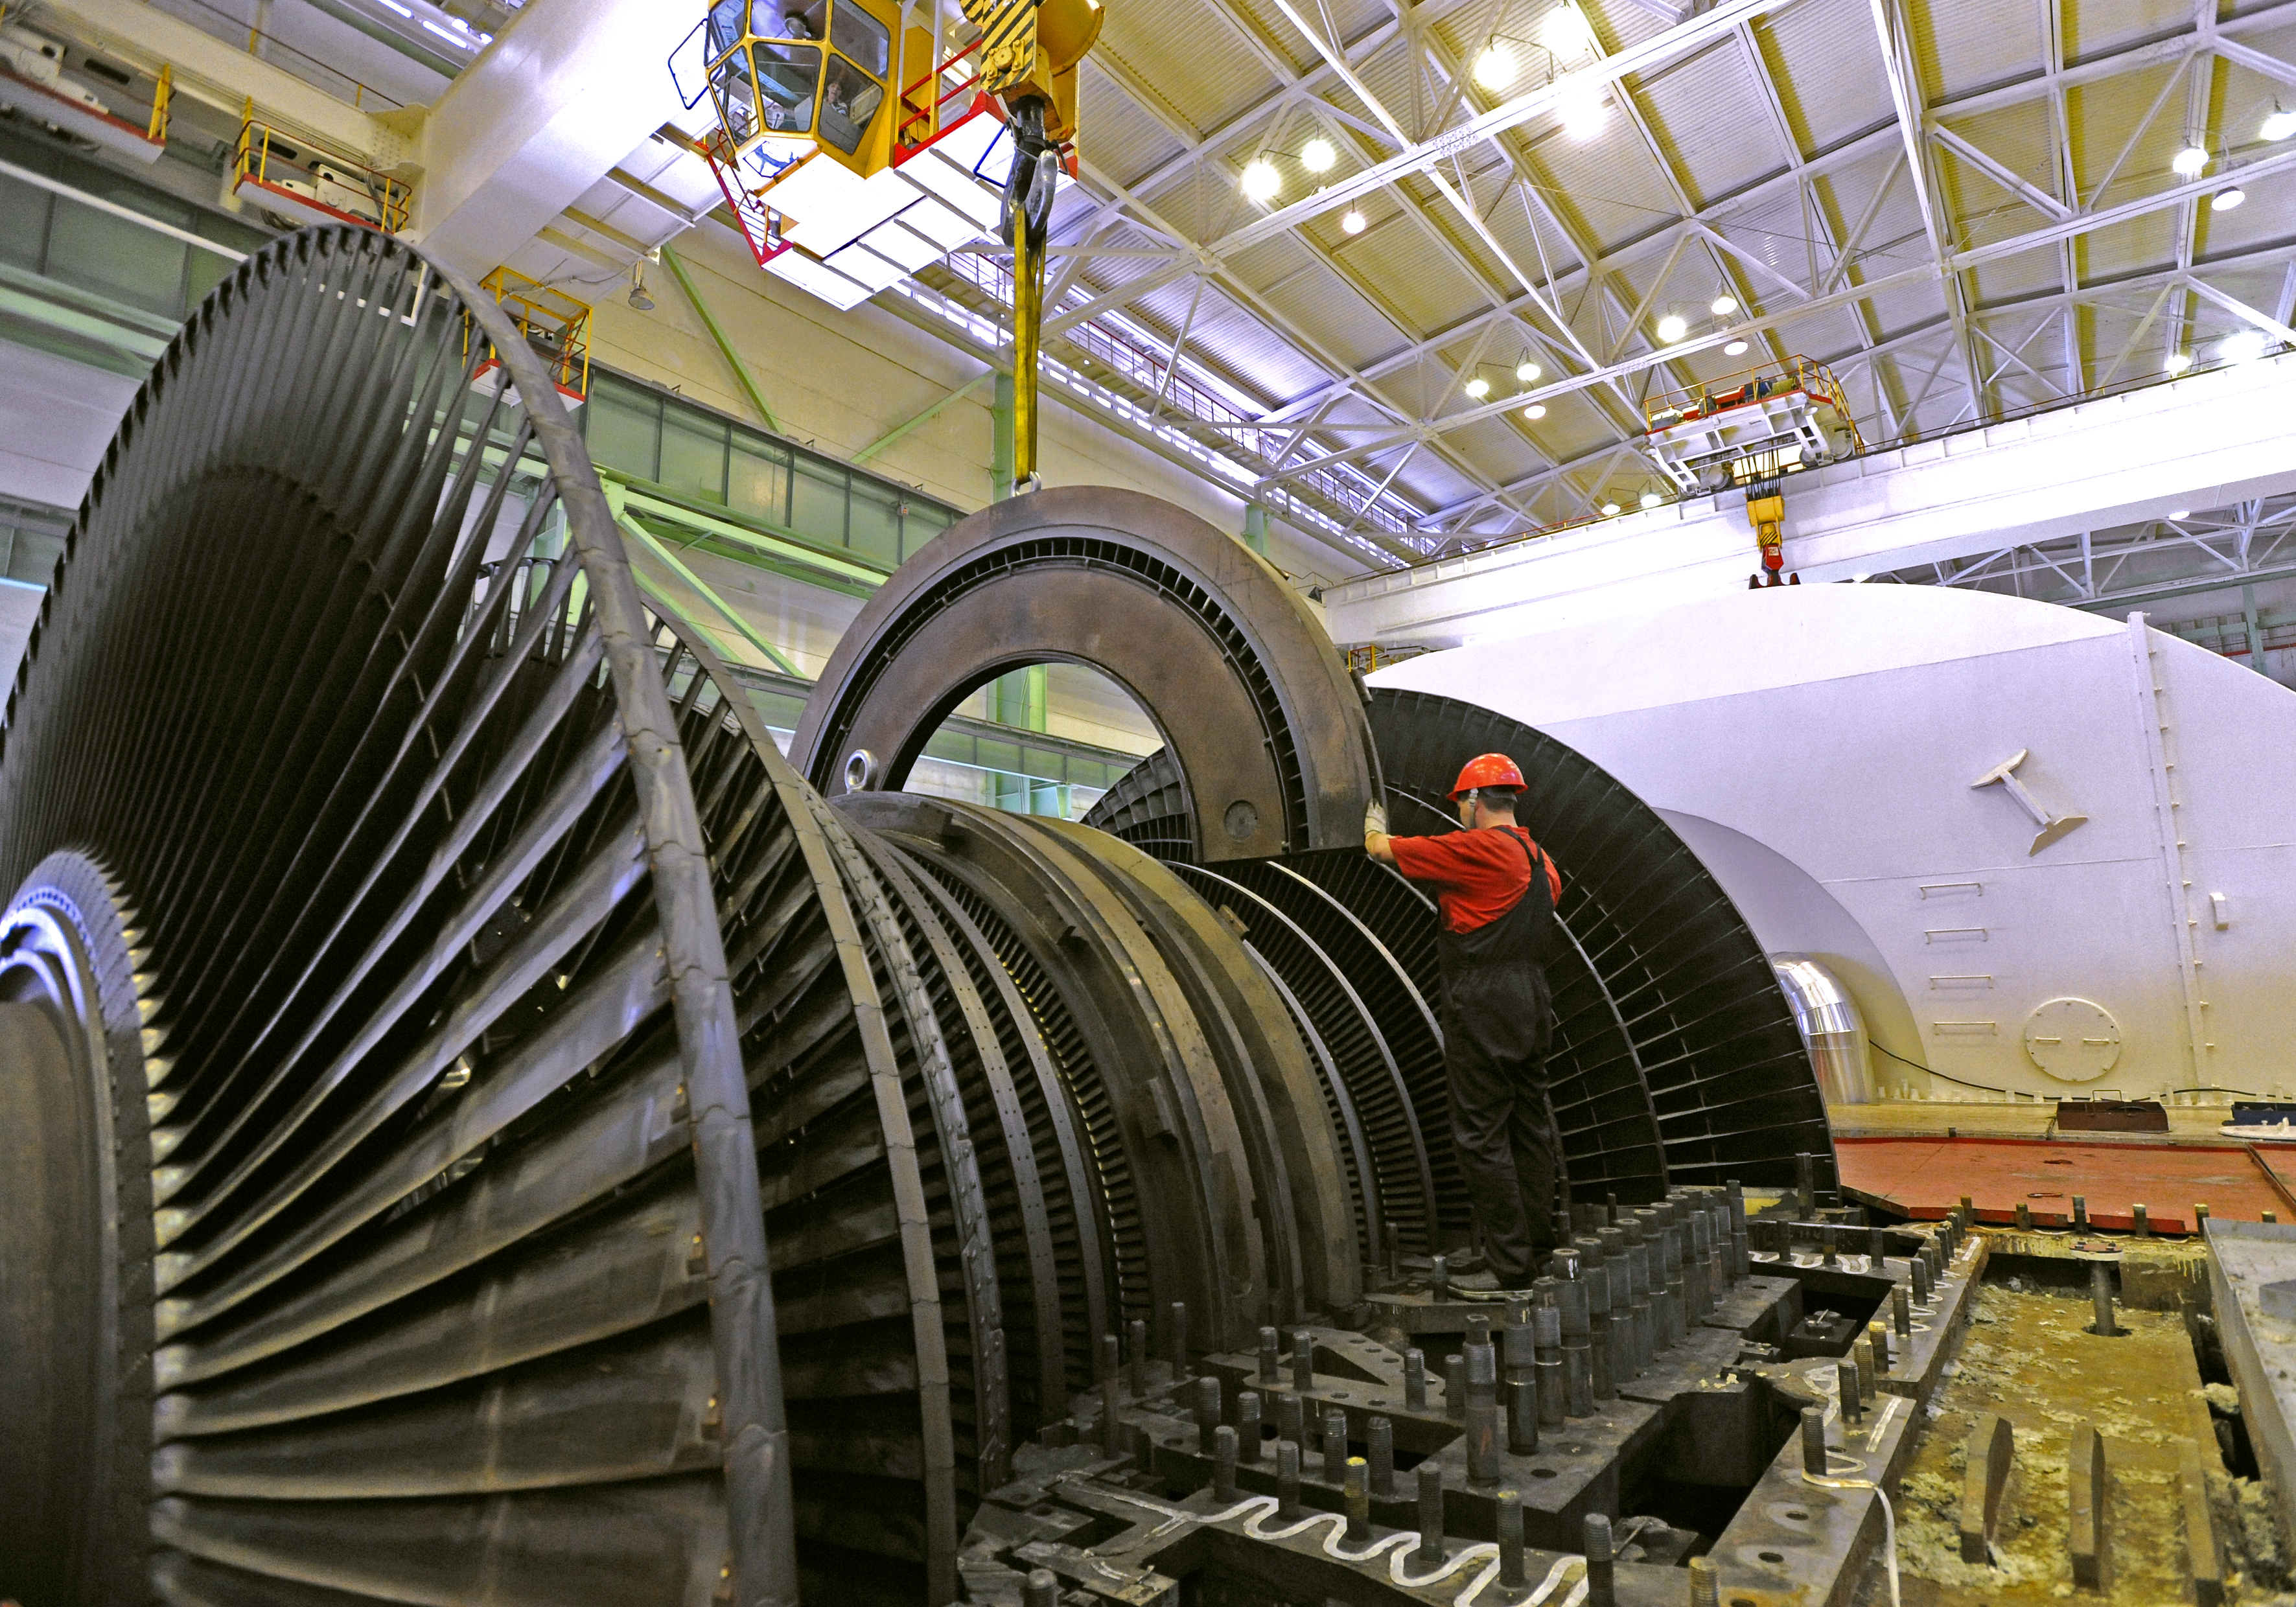
\includegraphics[width=14cm]{image/5-2-2.jpg}
\caption{俄罗斯巴拉科沃(Balakovo)核电站汽轮机}
\end{figure}

根据以上原理,\,热机主要分为以下两大类:
\begin{description}
	\item[\hei 蒸汽机(steam engine)]  蒸汽机是一类\emph{外燃机}(external combustion engines),\,工作物质是在气相与液相混合的水(水蒸气).\,用外界燃烧的热量,\,或者来自太阳能,\,核能,\,地热等的非燃烧热量加热\emph{锅炉}(boiler)中的水,\,由此产生高温高压蒸汽,\,用蒸汽带动机械装置运转向外输出能量.\,经过这样的装置后(这中间一般视为节流过程),\,水蒸气一般变为过饱和的冷气体或者还夹杂着水滴,\,进一步导入冷凝器而液化变为液态水回收进入锅炉.\,完成一个循环.\,18世纪末与大半个19世纪可谓``蒸汽时代'',\,蒸汽机在大型机械生产工厂,\,蒸汽机车,\,蒸汽机轮船等交通工具中大放异彩.\,虽然石油开采为小型汽车生产提供了可能,\,大型交通工具和生产业动力来源之后也慢慢地几乎被内燃机与电力所取代.\,但直到今天,\,我们的生产生活有$90\%$以上的电量都来自于\emph{汽轮机}(steam turbine)形式的热电厂.\,值得一提的是其中化石能源(煤电,\,气电,\,以及较为小规模的油电)仍然占据$75\%$的高比重(中国与美国的情况大致相同),\,新型能源的比重不大,\,但在稳步上升中.
	\item[\hei 内燃机(internal combustion machine)]  蒸汽机的锅炉设计让燃烧能量给了流动的工作物质,\,实现了工作物质不含燃料,\,不与燃料混合或被燃料污染.\,这有效地提高了燃料能量利用的效率.\,然而却需要为工作物质准备额外的空间,\,不利于把热机做小.\,与之相反,\,内燃机利用了\emph{燃烧室}(combustion chamber)的设计,\,工作物质直接是高能量密度的燃料和氧化剂(一般就是空气).\,利用高温高压下点燃化学反应释放的巨大化学能来产生热,\,导致气体反向对机械装置\ca \emph{活塞}(piston)或\emph{涡轮}(rotor)做功.\,与外燃机工作物质发生的真循环过程不同,\,内燃机发生的过程是一种开放循环.\,以常规的四冲程活塞式内燃机为例,\,气体经历四个冲程:\,\emph{吸入}(intake),\,\emph{压缩}(compression),\,\emph{做功}(power),\,\emph{排出}(exhaust).\,整个循环从常态燃料中开始,\,最后以排出气体在大气中冷却结束.\,而\emph{燃气涡轮发动机}(gas turbine engine)更是针对四个阶段分别设计功能区,\,使得四个阶段同时进行,\,提供了极大的功率输出.\,按照其机械装置的不同分为四类:\,军用战斗机往往采用\emph{涡喷发动机}(turbojet engine),\,而民航客机往往是\emph{涡扇发动机}(turbofan engine);\,运输机,\,巡逻机经常采用\emph{涡桨发动机}(turboprop engine);\,而直升机和其他陆上,\,海上交通工具则通过\emph{涡杆发动机}(turboshaft engine)将动力用传动轴导出.\,在这样的设计中,\,燃料产生的能量用来驱动涡轮带动整个装置大量吸入外界空气\footnote{火箭除外,\,它需要自备燃料与氧化剂.}并有效地压缩气体从而产生动力.\,涡轮转动的能量也正是很多民航飞机上电力的来源.
\end{description}
\begin{figure}[H]
\centering
\includegraphics[width=17cm]{image/5-2-3.png}
\caption{左:\,四冲程活塞内燃机;\,右:\,四类涡轮机}
\end{figure}

我们发现,\,将实际的热机抽象为前图\ref{fig:heat engine}那样的模型往往是过分地简单了.\,实际问题中的工作物质往往成分在发生改变,\,有物质的输入输出,\,甚至无法视为一个完整的循环过程.\,但理论可以帮我们分析与把握这个过程的一些主要信息.\,在实际问题中热机的\emph{能效}(energy efficiency)是主要的关心因素之一,\,它定义为输出的有用功$W$与燃料提供的化学能$Q_{\rm H}$之比:
\[\eta=\frac{W}{Q_{\rm H}}\]

\begin{wrapfigure}[22]{o}[-10pt]{7cm}
\centering
\includegraphics[width=7cm]{image/5-2-4.png}
\caption{热泵的普遍构成}
\vspace{1cm}
\includegraphics[width=7cm]{image/5-2-5.png}
\caption{热泵的工作循环}
\end{wrapfigure}
而热泵也根据其设计功能分为\emph{制冷机}(cooling machine),\,\emph{制热机}(heating machine)与\emph{可逆机}(reversible machine).可逆的热泵同时具备制冷制热两种功能,\,采用换向阀来控制气流的流向从而改变效果.\,当采用制热模式时,\,其效率往往比使用单独的电阻加热高3到4倍.

无论何种类型的热泵,\,其构成与原理可以被抽象为典型的四步.\,高温热源处更高温的气体在\emph{冷凝器}(condenser)处变为液态而放热;\,\emph{膨胀阀}(expansion valve)处的节流过程使液态流体温度与压强大降而成为气液混合的状态;\,低温冷库处稀薄的半液态流体在\emph{蒸发器}处蒸发吸热;\,最后通过\emph{压缩机}(compressor)泵入冷凝管,\,压强与温度显著升高.\,这样的循环称为\emph{斯特林循环}(Stirling cycle).


而对于热泵的\emph{性能系数}(coefficient of performance),\,需要对两种不同的模式区分:

对于制冷模式,\,取低温冷库处吸热比输入功率:
\[\eta=\frac{Q_{\rm L}}{W}\]

对于制热模式,\,取高温热源处放热比输入功率:
\[\eta=\frac{Q_{\rm H}}{W}\]

两者都可能大于一.

\subsection{热机循环}
从瓦特({\it Watt}\,)改良蒸汽机开始,\,一代代的工程师开始致力于提高热机的效率.\,这其中便产生了大量实用的热机模型.\,直到1824年法国物理学家与工程师卡诺({\it Carnot}\,)给出了惊人的卡洛热机模型与关于热机工作效率上限的论断.\,这实际上意味着\emph{热力学}(thermodynamics)的诞生.\,之后热机优化建立在严格的热力学计算的基础上.\,发展到今天理论早已成熟,\,只待技术的发展与革新.

简单的热机循环计算往往将工作物质视为理想气体在$p-V$图上的准静态过程构成的循环.\,下将一一列举:
\subsubsection{\hei 勒鲁瓦循环(Lenoir cycle)}
\begin{wrapfigure}[11]{o}[-10pt]{5cm}
\centering
\includegraphics[width=5cm]{image/5-2-6.png}
\caption{Lenoir cycle}
\end{wrapfigure}
1860年法国工程师勒鲁瓦发明的勒鲁瓦机是第一个为商业设计的内燃机.\,其对应循环常常用来描述\emph{脉冲喷气发动机}(pulse jet engine)的模型.\,它区别于其他热机的特点是无需压缩气体.\,一个循环内,\,理想气经历:
\begin{enumerate}[i]
	\item 1-2:\,定容爆炸吸热
	\item 2-3:\,绝热膨胀
	\item 3-1:\,定压放热
\end{enumerate}

定义\emph{爆炸比}(explosion ratio)$r_p$:
\[r_p=\frac{p_2}{p_1}\]

则可以计算出其效率为:
\[\eta=1-\gamma\frac{T_3-T_1}{T_2-T_1}=1-\gamma\frac{r_p^{\frac{1}{\gamma}}-1}{r_p-1}\]
\subsubsection{\hei 奥托循环(Otto cycle)}
\begin{wrapfigure}[12]{o}[-10pt]{5cm}
\centering
\includegraphics[width=5cm]{image/5-2-7.png}
\caption{Otto cycle}
\end{wrapfigure}
这是最典型的四冲程型\emph{汽油机}(gasoline engine,\,gas engine)的工作循环.\,特点是通过压缩气体产生高温高压易燃汽油空气混合体,\,再通过火花塞点燃混合体,\,过程可以视为瞬间发生的,\,从而体积不变,\,压强突然增大.\,一个循环内,\,理想气经历:
\begin{enumerate}[i]
	\item 1-2:\,绝热压缩
	\item 2-3:\,定容爆炸吸热
	\item 3-4:\,绝热膨胀
	\item 4-1:\,定容放热
\end{enumerate}

定义\emph{压缩比}(compression ratio)$r$:
\[r=\frac{V_1}{V_2}\]

则可以计算出其效率为:
\[\eta=1-\frac{T_1}{T_2}=1-\frac{T_4}{T_3}=1-r^{-(\gamma-1)}\]

对于空气与燃油的混合气$\gamma\simeq 1.3$,\,由于爆炸燃烧机制,\,目前的压缩比能做到$r\simeq 10$,\,这样看其理论效率上限$\sim 50\%$,\,目前一般的汽油机效率为$25\%\sim35\%$.\,最高能到$40\%$,\,离理论上限还尚有一段提升空间.

\npg{0cm}

\vspace{1cm}

\subsubsection{\hei 迪塞尔循环(Diesel cycle)}

迪塞尔机又称为\emph{柴油机}(Diesel fuel engine).\,其与汽油机设计上存在区别.\,为了提高汽油机的效率,\,柴油机企图增大压缩比,\,故采用粗重的活塞.\,并取消汽油机中点火爆炸的过程,\,而让压缩冲程的末温直接使得燃料能够燃烧,\,而缓慢注入燃料以使得燃烧充分.\,这样,\,典型的迪塞尔循环可以认为是这样四个过程:
\begin{wrapfigure}[12]{o}[-10pt]{5cm}
\centering
\includegraphics[width=5cm]{image/5-2-8.png}
\caption{Diesel cycle}
\end{wrapfigure}
\begin{enumerate}[i]
	\item 1-2:\,绝热压缩
	\item 2-3:\,定压燃烧吸热
	\item 3-4:\,绝热膨胀
	\item 4-1:\,定容放热
\end{enumerate}

定义压缩比$r$与\emph{停气比}(cut off ratio)$\alpha$:
\[r=\frac{V_1}{V_2}\quad ;\quad \alpha=\frac{V_3}{V_2}\]

则可以计算出其效率为:
\[\eta=1-\frac{1}{\gamma}\cdot\frac{T_4-T_1}{T_3-T_2}=1-\frac{\alpha^\gamma-1}{\gamma r^{\gamma-1}(\alpha-1)}\]

\vspace{2cm}

\subsubsection{\hei 布莱顿循环(Brayton cycle)}

涡轮机等开放式热力学循环的一般抽象是带有两个等压过程的布莱顿循环.\,可以认为是这样四个过程:
\begin{wrapfigure}[12]{o}[-10pt]{5cm}
\centering
\includegraphics[width=5cm]{image/5-2-9.png}
\caption{Brayton cycle}
\end{wrapfigure}
\begin{enumerate}[i]
	\item 1-2:\,绝热压缩
	\item 2-3:\,定压燃烧吸热
	\item 3-4:\,绝热膨胀
	\item 4-1:\,定压放热
\end{enumerate}

定义\emph{压强比}(pressure ratio)$r_p$:
\[r_p=\frac{p_2}{p_1}\]

则可以计算出其效率为:
\[\eta=1-\frac{T_1}{T_2}=1-{r_p}^{-\frac{\gamma-1}{\gamma}}\]

\npg{-3cm}

\subsubsection{\hei 卡诺循环(Carnot cycle)}

卡诺循环是一种具有极其重要的理论意义的理想循环.\,它不能对应实际应用与生活与生产的实际热机.\,但是却像直线与平面之于几何理论那样,\,对卡洛循环与热机的很多讨论都将与热力学理论体系紧密相关.\,对于理想气体,\,卡诺循环意味着其吸放热都发生在与两个恒温热源做等温接触的过程中.
\begin{wrapfigure}[10]{o}[-10pt]{5cm}
\centering
\vspace{-0.5cm}
\includegraphics[width=5cm]{image/5-2-10.png}
\caption{Carnot cycle}
\end{wrapfigure}
整个循环由两条绝热线与两条等温线围成.\,过程如下:

\begin{enumerate}[i]
	\item 1-2:\,绝热压缩
	\item 2-3:\,等温吸热
	\item 3-4:\,绝热膨胀
	\item 4-1:\,等温放热
\end{enumerate}

高温热源的温度为$T_{\rm H}$,\,低温冷库的温度为$T_{\rm L}$.\,那么可以计算出卡诺热机的效率为:
\[\eta=1-\frac{T_{\rm L}}{T_{\rm H}}\]


\section{理想气体的熵}

理想气体的准静态过程是这一章内我们关心的问题.\,如何判断一个微元准静态过程中理想气体吸热还是放热?\,具体来说,\,我们关心在$(T,\,V)$点沿着$(\ud T,\,\ud V)$变化方向改变状态所需要吸收的热量微分$\dbar Q$.\,由热一,\,它应为:
\[\dbar Q=\ud U+p\ud V=\nu C_{mV}\ud T+\frac{\nu RT}{V}\ud V\]

这可以进行如下的化简:
\[\dbar Q=\nu C_{mV} T\cdot [\frac{\ud T}{T}+(\gamma-1)\frac{\ud V}{V}]=\nu C_{mV} T\cdot\ud \ln(TV^{\gamma-1})\]

我们定义态函数\ca \emph{熵}(entropy):
\[S_1=\nu C_{mV}\ln(TV^{\gamma-1})\]

那么自然得出:
\[\dbar Q=T\ud S_1\]

这给出了气体吸放热与状态变化之间的联系.\,一个直接的推论就是,\,准静态绝热过程中$TV^{\gamma-1}$是不变的(绝热方程).\,或者说,\,准静态绝热过程可以被称为\emph{等熵过程}(isentropic process).\,而熵作为一个态函数,\,等熵线就是绝热线.

熵在定义时可以相差一个与状态无关的常数(但与摩尔数$\nu$有关,\,目前它不随着状态变化而变化).\,我们为了方便暂时不写这个常数.\,但如果我们一开始以$(p,\,V)$或者$(p,\,T)$作为状态参量.\,那么自然而然写出来的符合$\dbar Q=T\ud S$的熵为:
\[S_2=\nu C_{mV}\ln(pV^\gamma)\quad ;\quad S_3=\nu C_{mV}\ln\frac{T^\gamma}{p^{\gamma-1}}\]

它们都相差一个过程不变的常数:
\[S=S_3\quad ;\quad S_1=S+\nu R\ln(\nu R)\quad ;\quad S_2=S+\nu C_{mp}\ln(\nu R)\]

我们把$S_3$取为标准的熵.\,原因在于,\,如果我们要讨论摩尔数$\nu$变化的情况时.\,在对数里放两个强度量可以使表达式成为一个广延量\ca 当摩尔数增大到$\lambda$倍而所有强度量不变时,\,熵$S$也增大到$\lambda$倍.\,而其他两个$S$附加的项$\nu R\ln(\nu R)$与$\nu C_{mp}\ln(\nu R)$使得定义失去了这种广延性.

\begin{figure}[H]
\centering
\includegraphics[width=15cm]{image/5-2-11.png}
\caption{左:\,吸放热的元过程方向;\,右:\,两根等熵线间的``热量差''}\label{fig5-2-11}
\end{figure}

我们由此得出这样的结论:\,在一个准静态过程中.\,沿着等熵线以下的方向熵降低(如图\ref{fig5-2-11}中蓝色箭头方向),\,从而要放热.\,而往上走则熵增加,\,要吸热.\,但注意到既使沿着切线方向走熵还是会降低(无论往上还是往下),\,只不过这时候其降低是一个二阶小量而已.\,也就是说如果气体历经$p-V$图上的负斜率直线过程,\,一定是先吸热,\,后放热.\,在中间有一个熵的极值点符合:
\[k=\frac{\ud p}{\ud V}=-\gamma\frac{p}{V}\]

我们画出两条相隔很近的等熵线(差$\ud S$).\,注意到两条线之间的``热量差''这个概念本身不够严谨,\,因为热量是过程量不是状态量.\,但由于两条等熵线相隔很近,\,所以从一点出发到另一条绝热线上的点还在这一点附近(微元过程,\,取$\Delta S\rightarrow 0$的极限).\,所以可以认为温度近似不变.\,尽管这样,\,吸热仍然与过程发生的平均温度$T$有关:
\[Q_{\rm H}=T_{\rm H}\ud S\quad;\quad Q_{\rm L}=T_{\rm L}\ud S\]

\begin{figure}[H]
\centering
\includegraphics[width=15cm]{image/5-2-12.png}
\caption{示功图与示热图}\label{fig5-2-12}
\end{figure}

由于$S$是态函数,\,我们也可以选取$(T,\,S)$来作为体系的状态参量.\,而做$T-S$图表示状态与过程.\,此时等温线实际上就是水平线,\,而绝热线就是竖直线.\,而其包围的面积实际上就是整个过程所吸收的热量:
\[Q=\oint T\ud S\]

而由于热一,\,它一定等于$p-V$图中的面积,\,它表示对外做功:
\[W=\oint p\ud V\]

正是由于这个直观的关系,\,热力学理论分析时我们经常对照两个图像.\,分别叫做\emph{示功图}(work indicator diagram)与\emph{示热图}(heat indicator diagram).

还有两点值得讨论:

第一,\,以上讨论仅仅限于理想气体的准静态过程.\,我们发现对于理想气体,\,如果采用理想气体温标(即分子内能恰正比于温度),\,恰好可以引入独特的态函数熵来计算其吸热.\,然而,\,对于非准静态过程初末态之间的联系我们还一无所知,\,仅仅知道热一总是成立的.

第二,\,对于其他体系是否有$\dbar Q=T\ud S$?,\,这看上去似乎不显然.\,首先我们知道热力学第零定律定义了温度是某种热平衡的系统共同具有的属性,\,但我们一直使用的温度似乎是根据理想气体的分子平均动能定义出来的(理想气体温标):


这样,\,直接把这个温度用于其他体系似乎不太可能会得出相似的结论,\,而另外定义新的温标又会造成物理规律的不统一性.\,温度也就失去了作为了互为热平衡态共同参数的性质.\,然而,\,需要知道上式不是无来由的,\,它来源于麦克斯韦分布律\ca 微观体系的经典动力学与统计规律的共同结果,\,在这一点上其实温度的定义是普适的,\,它都反应了各个自由度上热运动的剧烈程度.\,所以实际上存在普适的热力学温标,\,而同样的也将存在对应的普适的态函数熵.\,它们都由大量微观粒子的统计规律给出.\,然而十分神奇的一点是,\,普适的温度与熵的存在性在历史上和逻辑上的确是可以由简单的公理得出的热力学第二定律的体系.\,这正是下一节我们要说明的.\,而要深刻了解温度与熵的微观本质需要深入了解统计力学方法,\,我们在下一章将给出相关的论述.
\[T=\frac{2\overline{\varepsilon_k}}{3k}\]


\section{热力学第二定律}

费曼说过,\,所有自然现象的最自然特征莫过于它们明显的不可逆性.\,大量微观粒子构成的宏观热力学体系在种种现象上体现出不可逆的特性,\,即\emph{热力学时间箭头}(time arrow of thermodynamics).\,如果令时间反演,\,系统的各状态逆序发生,\,外界对其做功变为对外做功,\,向外界放热变为从外界吸热.\,那么很多现象都给出了从未被观察到的结果:\,混合均匀地两钟气体自发地分开,\,低温冷库向高温热源自发放热,\,热能单一地转化为机械能等等.\,无耗散的准静态过程是理想的\emph{可逆过程}(reversible process),\,仅有系统内部处处达到细致平衡,\,在与外界平衡的状态下统一地改变其状态才能将其过程反演而符合物理规律.\,而广泛存在的\emph{不可逆过程}(reversible process),\,一方面在于过程反演的不实际性,\,还在于如果我们把系统和外界各部分视为一整个孤立的体系,\,那么发生的不可逆过程无法通过任何可能的过程回到初始状态.\,在发生不可逆过程的时候,\,体系的某些特征沿着一个方向被永久而不可恢复的改变了,\,衡量这个特征的物理量就是熵,\,而这种断言就是热力学第二定律.\,它回答了热一所不能回答的问题,\,给出了热力学过程发生的方向性与限度.\,对于这些问题的讨论是热二的特色.

热力学第二定律在逻辑体系上承接热力学第零,\,第一定律,\,我们现在取消前面已经有良好定义的理想气体与针对它的温标的概念.\,而热机模型与其效率只取决于吸放热仍然有良好的定义:
\[\eta=1-\frac{Q_{\rm L}}{Q_{\rm H}}\]

\begin{figure}[H]
\centering
\includegraphics[width=15cm]{image/5-2-13.png}
\caption{熵增原理}\label{fig5-2-13}
\end{figure}
我们讨论一个$p-V$系统作为工作物质在两个恒温热源(冷库在此被称为低温热源)之间的工作,\,各个温度暂时只是一个记号,\,其值暂不确定.\,为了统一起见,\,我们研究系统与外界的功热交换时规定$\ud U=\dbar W+\dbar Q$,\,即以从外界吸热和外界对其做功为正.\,首先,\,我们孤立那个$p-V$系统,\,让它做绝热过程而只能与外界有功的交换.\,那么准静态的绝热过程\footnote{它具有极其独特的含义,\,参见之后第五章的讨论.}将给出系列绝热线,\,它们彼此绝不可以相交,\,否则在一点处将存在多个绝热的方向.\,图中为了简化而近似画成了平行直线(这在微元的循环过程中\ca 微小吸放热,\,微小温差\ca 是合理的处理方法).\,现在考虑一个非准静态的绝热过程.\,如果是绝热压缩,\,那么外界给予气体的压强应该大于系统的平均压强,\,这样造成的不平衡才可以使得系统自发收缩.\,如果是绝热膨胀,\,同理,\,外界给予气体的压强应该小于系统的平均压强.\,不管怎样,\,都有:
\[\dbar W \geq -p\ud V\]

这样造成的结果是系统的状态只能往绝热线的一侧走,\,类似于热力学第零定律,\,对于这个特定体系,\,我们暂时可以把这些可以通过准静态绝热过程相互连接的状态称为具有共同的熵.\,而更高的绝热线代表更高的熵,\,以上观点给出了\emph{熵增原理}(principle of entropy increase):

\begin{center}
\hei 熵增原理:\,孤立系统的熵只增不减,\,$\Delta S \geq 0$
\end{center}

这一点的意义不仅仅在于末态到达另一条绝热线上以后仍然孤立地自发回到初始状态,\,还意味着既使借助外界\ca 两个恒温热源,\,可能出现的其他辅助工作物质的帮助,\,也无法在不改变其他物体的状态(两个热源净吸放热为零,\,其他工作物质初末状态复原)的条件下回到初始状态,\,原来的功也被补偿.\,这构成热力学第二定律的一种表述,\,它在热力学体系里是公理,\,代表了自然界的某种规律.

\begin{figure}[H]
\centering
\includegraphics[width=15cm]{image/5-2-14.png}
\caption{三种不可逆过程的联系}\label{fig5-2-14}
\end{figure}

质疑这一点会引发什么结果?\,如果在某个任意中间温度$T,\,T_{\rm L}<T<T_{\rm H}$下可以通过某个过程让较高绝热线上的状态回到相距很近的较低绝热线上的状态.\,那么我们将它与两条绝热线和在低温热源上吸热膨胀的过程组成一个循环,\,其合效果是从低温热源吸收了热,\,并完全转变为对外界的做功.\,这也是被热力学第二定律禁止的,\,或者说其反过程不可逆:

\begin{center}
\hei 开尔文表述:\,功变热不可逆,\,$W=-Q\geq 0$
\end{center}

表述为文字,\,则为热机不可能在一个循环过程中从单一热源吸热转变为对外做功而不产生其他影响.

继续质疑这一点.\,再构造一个热泵B,\,它接受来自热机A的功而从低温热源向高温热源泵热,\,其总结果是,\,低温热源向高温热源传了热,\,其他体系状态历经一个循环回到初态.\,同样的,\,它被热力学第二定律禁止:

\begin{center}
\hei 克劳修斯表述:\,温差传热不可逆,\,$Q_{\rm H}=-Q_{\rm L}\geq 0$
\end{center}

可见热力学第二定律的不同表述之间都是相互联系的.\,实际上如果把两个热源和工作物质视为整体,\,那么其实后两个表述就是整个体系的熵增原理,\,此时,\,整个循环过程来看,\,如果过程中时时,\,处处都是无耗散的准静态过程,\,那么熵应该是不变的,\,过程应该是可逆的,\,这就是卡诺热机模型:\,是高温热源与气体等温时放热$Q_{\rm H}>0$,\,气体与低温热源等温时再放热$|Q_{\rm L}<0|$.\,而气体对外做功为$|W=-Q_{\rm H}-Q_{\rm L}<0|$.\,或者是这个过程的逆过程\ca 卡诺热泵循环.\,对于所有热机,\,热力学第二定律断言:

\begin{center}
\hei 卡诺定理:\,卡诺热机效率最高,\,$\displaystyle \eta=1-\frac{-Q_{\rm L}^\prime}{Q_{\rm H}^\prime}\leq 1-\frac{-Q_{\rm L}}{Q_{\rm H}}$
\end{center}

证明思路是,\,如果有热机效率高于卡诺热机效率,\,意味着输出相同的功时其在两个热源的吸放热可以同时减到比卡诺热机小,\,那么用输出的功给一个对应的卡诺热泵,\,总的结果是低温热源向高温热源放热了,\,由于热力学第二定律,\,这不可以成立.

从而,\,卡诺定理实际上也是热力学第二定律的等价表述.\,这些表述都有一个特点,\,可逆过程对应取等号,\,而不等号发生在不可逆的过程中,\,代表过程的方向性.\,在等号情况下,\,工作于两个恒温热源间的可逆卡诺热机的吸放热比是恒定的,\,这给出了热力学温标的定义:
\[\frac{-Q_{\rm L}}{Q_{\rm H}}=\frac{T_{\rm L}}{T_{\rm H}}\]

只需确定一种特定系统的温度,\,便可以由可逆循环的吸放热比测量任意其他平衡态的温度.\,目前,\,这种特定的系统被取做水的三相共存系统\footnote{2018年预通过的新国际单位制提案指出将可能把联系微观统计规律与宏观测量的常数$k_B$作为基本常数.\,这样确定了温度与能量换算的线性关系,\,从极低温到极高温完全一致.},\,温度定义为$273.16{\rm K}$.\,这就是热力学温标.\,而这也给出了与之共轭的熵的概念:
\[\ud S=\frac{\dbar Q}{T}\]

上式对可逆过程适用.\,对于卡诺循环来说,\,如果着眼点在整个系统,\,那么一个循环下来工作物质的熵是复原的.\,而两个恒温热源的熵变根据上面温度的定义:
\[\Delta S=-\frac{Q_{\rm H}}{T_{\rm H}}-\frac{Q_{\rm L}}{T_{\rm L}}=0\]

可见大的系统初末态在一条等熵线(实际上整个循环中每一个状态之间都彼此等熵,\,因为整个系统做绝热可逆过程)上.\,而如果我们着眼点在气体上,\,而且让气体做一个任意的可逆循环过程,\,一定有:
\[\Delta S=\oint \frac{\dbar Q}{T}=0\]

以上式子为克劳修斯等式(Clausius equality),\,同理对于不可逆过程将给出不等式,\,普遍的,\,我们对一个系统,\,有:
\[\Delta S=S_{\rm final}-S_{\rm initial}\geq \int_{\rm initial}^{\rm final}\frac{\dbar Q}{T}\]

上式也是热力学第二定律的表述,\,它十分强大,\,其他表述都可以简单地从这个表述验证.\,它甚至有十分清晰的图像:\,右边是从外界流向系统的熵流,\,左右的区别在于系统内部不平衡条件下的各种流造成的熵产生,\,详见下一节和本章最后一节的相关讨论.\,对于上式,\,如果不等号左边为零,\,可以理解为功变热的不可逆性:\,右边积分里的$\dbar Q$小于零将使得不等式成立,\,说明在过程中体系更自发的行为是接受外界对其做功,\,而以放热的形式形成能量守恒,\,当然条件是初末态等熵\ca 一般考虑循环过程.\,如果不等式右边为零,\,给出了熵增原理\ca 绝热体系的熵只增不减.



\vspace{1cm}
\section{熵的计算}

\subsection{理想气体的熵}

理想气体温标与热力学温标为何统一?\,一者,\,用理想气体温标定义的温度自动符合卡诺定理:\,卡诺循环效率为热力学定义值$\displaystyle\eta=1-\frac{T_{\rm L}}{T_{\rm H}}$,\,且关键是它能使得下式成为全微分:
\[\ud S=\frac{\dbar Q}{T}=\frac{\ud U+p\ud V}{T}=f(T,\,V)\ud T+g(T,\,V)\ud V\]

如果理想气体温标是$T'=h(T)\cdot T$,\,那么$\displaystyle \frac{\dbar Q}{T'}$不可能再是一个全微分,\,而与热力学第二定律定义的温标不一致.\,

二者,\,热力学第二定律的体系看似复杂而充满精巧的构造,\,实则可以在更深的层次:\,微观动力学规律与统计规律的基础上进行自然的推导.\,此时温度,\,熵,\,热量不仅可以普适而简单地定义,\,而且具有清晰的物理图像,\,我们在第五章统计物理基础中展开说明.

所以,\,理想气体的熵我们可以直接使用第二节的推导,\,不过我们这里写作:
\[S(T,\,V)=\nu C_{mV}\ln T+\nu R \ln V\]
\[S(p,\,V)=\nu C_{mV}\ln p+\nu C_{mp} \ln V\]
\[S(p,\,T)=\nu C_{mp}\ln T-\nu R \ln p\]

以上三个定义不太一样,\,差一些取决于摩尔数$\nu$的常数.\,而且只有最下面一个是广延量.\,一种常见的处理方法是把体积换为摩尔体积:
\[V_m=\frac{V}{\nu}\]

摩尔体积实际上与比体积(单位质量的体积)$v$,\,密度$\rho$,\,粒子数密度$n$有如下正反比关系:
\[\rho=\frac{1}{v}=\frac{\mu}{V_m}=nm\]

这样三个式子都变成了广延量.\,它们还差一些与$\nu$成正比,\,对数里面是$R$的一些广延量.\,这种定义的非唯一性很正常,\,实际过程中产生实际效果的是熵的变化量,\,仅有在极低温下,\,讨论量子体系时才需要讨论熵的绝对数值(热力学第三定律).\,还有一点,\,为了使得对数里的物理量不带单位,\,我们规定$p=p_0,\,v=v_0,\,T=T_0$时的熵为零,\,最后得到统一的熵的公式:
\[S=\nu C_{mV}\ln \frac{T}{T_0}+\nu R \ln \frac{v}{v_0}=\nu C_{mV}\ln \frac{p}{p_0}+\nu C_{mp} \ln \frac{v}{v_0}=\nu C_{mp}\ln \frac{T}{T_0}-\nu R \ln \frac{p}{p_0}\]

熵是广延量,\,我们作此要求.\,说明我们可以将一个均匀的系统按某比例分成若干份,\,熵也会随之分成对应比例的份数.\,甚至,\,我们可以将上面的熵除以总分子数,\,得到每一个分子上的熵的结果:
\[\varsigma=\left( \frac{i}{2}+1 \right)k\ln T-k\ln p \]

乍一看这是荒诞的,\,一个分子具有能量可能还比较好理解,\,但是一个分子为何可以具有温度,\,压强,\,甚至熵的概念?\,这些问题需要等我们之后章节研究了熵的统计学和信息学含义以后才能理解.

\subsection{固定热容固体熵}

理想情况下这种固体是以温度为单参数热力学系统,\,其内能为
\[U=CT\]

而吸热就是$Q=C\Delta T$,\,从而熵:
\[dS=C\frac{\ud T}{T}\]

从而:
\[S=C\ln\frac{T}{T_0}\]

\subsection{大热容恒温热库}

无疑,\,这种情况是上一种情形的大热容极限近似,\,如果温度变化$\Delta T$相对于$T$很小:
\[\Delta S=C\ln\frac{T+\Delta T}{T}\simeq\frac{C\Delta T}{T}=\frac{\Delta U}{T}\simeq\Delta{\frac{U}{T}}\]

即此时等价的定义不会造成区别:
\[S=\frac{U}{T}\]

\subsection{传热熵}

\begin{wrapfigure}[14]{o}[-10pt]{6cm}
\centering
\vspace{-0.5cm}
\includegraphics[width=6cm]{image/5-2-15.png}
\caption{传热熵产生}
\end{wrapfigure}
如果高温物体温度$T_{\rm H}$,\,低温物体温度$T_{\rm L}$,\,两者发生一个热接触而有热流$\dbar Q$从高温物体流向低温物体.\,这是一个非准静态过程,\,它不可逆,\,如何分析其熵的呢?\,考虑高温物体放热$\dbar Q$,\,实际上如果它是与一个温度同为$T_{\rm H}$的恒温热库接触而放出这个热量,\,其状态的改变是完全相同的,\,不过这是一个准静态过程,\,可以计算其熵变:
\[\ud S_{\rm H}=-\frac{\dbar Q}{T_{\rm H}}\]

即,\,有$|\ud S_{\rm H}|$的熵从高温物体中流了出来.\,同理,\,流向低温物体的熵为:
\[\ud S_{\rm L}=\frac{\dbar Q}{T_{\rm L}}\]

整个体系熵要增加:
\[\ud S=\dbar Q(\frac{1}{T_{\rm L}}-\frac{1}{T_{\rm H}})> 0\]

上式被称为传热过程中的\emph{熵产生}(entropy production).\,它其实也代表某种微观形式的耗散,\,它发生于高温与低温物体接触时平均起来高温的动能较大的粒子动能被拉低而低温物体动能被拔高的过程中.

\subsection{混合熵}

讨论理想气体的混合,\,而且混合后各种气体分子间亦无任何形式的相互作用.\,命气体的第$i$组分的摩尔分数为$x_i$,\,混合前不同气体处于温度为$T$,\,压强为$p$的平衡,\,不同组分占体积比为:
\[V_1:V_2:\,\cdots\, :V_n=x_1:x_2:\,\cdots\,:x_n\quad ; \quad V_i=x_i V\]

混合后温度仍然是$T$,\,体积倒是共用一个$V$了.\,而不同组分去对$p$进行分压:
\[p_1:p_2:\,\cdots\, :p_n=x_1:x_2:\,\cdots\,:x_n\quad ; \quad p_i=x_i p\]

\begin{wrapfigure}[15]{o}[-10pt]{5cm}
\centering
\vspace{-0.5cm}
\includegraphics[width=5cm]{image/5-2-16.png}
\caption{混合熵}
\end{wrapfigure}
熵是广延量,\,混合理想气体的熵满足\emph{吉布斯定理}(Gibbs' theorem):\,混合气体的熵等于所有组分的熵的和,\,而每一组分在与其他组分共存的过程中,\,其他组分对这个组分可能的微观状态形式并无影响(分子间无相互作用).\,所以这个组分的熵就等于它单独存在时的熵.\,那么过程前后的熵变其实也就是气体向真空自由膨胀的熵变(因为$T$恰好不变,\,与自有膨胀特征相同),\,这是一个典型的不可逆过程:
\[\Delta S_i=\nu_i R\ln\frac{V}{V_i}=-\nu R x_i\ln x_i\]

故算出\emph{混合熵}(entropy of mixing)为:
\[\Delta S=-\nu R\sum x_i\ln x_i>0\]

我们写出末态混合均匀后熵的表达式,\,注意为了保证其广延性,\,我们采用$p,\,T,\,x_i$这些强度量作为其可以放到$\ln$后面的自变量:
\begin{eqnarray*}
S 	&=&	 \sum S_i \\
	&=&	\sum \nu_i C_{mp}\ln T-\nu_i R\ln p_i \\
	&=&	\nu C_{mp}\ln T-\nu R\ln p-\nu R\sum x_i\ln x_i \\
	&=&	S_0 +\Delta S
\end{eqnarray*}

从中混合熵的概念就十分明显了:\,它代表混合气体与同样条件下的单组分气体的熵$S_0$的区别.\,这很自然地引入了所谓的\emph{吉布斯佯谬}(Gibbs' paradox):\,一是为什么吉布斯定理不适用于单组分气体,\,如果把一缸气体体积分成两份,\,那么熵可以直接相加(广延性),\,但不能把这缸气体的压强(粒子数)分成两份而占据相同的体积,\,除非分成的两份分子有本质的不同.\,二就是多组分与单组分的区别在哪里,\,会造成物理量的差别.

这其实不是奇怪的事.\,我们考虑一缸氢气,\,它的熵应根据$S_0$计算,\,用它计算也符合测量结果.\,而某一天科学家们突然得知,\,原来氢分子${\rm H_2}$分为两种:\,核自旋平行的\emph{正氢}(orthohydrogen)和核自旋反向的\emph{仲氢}(parahydrogen),\,两者占比为$3:1$.\,两种分子仅仅是深入到原子核的性质略有不同,\,对常温下的分子物理化学性质几乎没有影响\footnote{然而低温下影响巨大,\,这与量子效应有关}.\,于是似乎要在熵公式后附加一项混合熵$\displaystyle -\nu R(\frac{1}{4}\ln\frac{1}{4}+\frac{3}{4}\ln\frac{3}{4})\approx 0.56\nu R$.\,这一项如何解释?\,通过第五章的学习我们将知道,\,熵实际上对应着信息的多少.\,在混合氢情况下我们知道了更多的信息:\,每一个氢分子究竟是正氢还是仲氢.\,所以熵增加了.\,但加这一项有必要吗?\,其实是没有必要的,\,因为它作为常数,\,在公式$\dbar Q=T\ud S$中求变化量时不出现,\,从而不会出现在实际可以测量的系统发生的过程中的宏观物理量上.\,然而一涉及到微观构成,\,它就是必要的了,\,如果两种氢之间可以相互转化,\,那么如果整缸氢气都是正氢或是仲氢,\,在一定时间后它将在两种氢之比为$3:1$处平衡,\,这个过程是个不可逆过程.\,这是因为正氢又分为三种可能的自旋态,\,那么把这三个态与仲氢的摩尔分数记做$x_1,\,x_2,\,x_3,\,x_4$,\,有:
\[x_1+x_2+x_3+x_4=1\]
\[\Delta S=-\nu R\ln\sqrt[4]{x_1x_2x_3x_4}\]

由算术几何平均不等式,\,在$\displaystyle x_1=x_2=x_3=x_4=\frac{1}{4}$处熵增取极大值.\,在这个状态往任何一个其他状态熵必然减少而不被热二允许.\,它就是我们要求的平衡态.\,所以两种氢之比为$3:1$,\,同时我们还可以看出之前我们算的熵变还不够严格,\,考虑四种氢时混合熵应为
\[\Delta S=\nu R\ln 4=1.4\nu R\]

值得一提,\,我们上面反过来通过预先在非平衡态都有良好定义的熵的极值来求平衡状态的参数条件的方法称为\emph{最大熵原理}(principle of maximum entropy),\,这种目前看似难以理解的方法亦会在第五章给出详细论述.



\section{热力学函数与其特性}

\subsection{四个热力学函数与四个状态参量}

在本节中我们将把态函数熵$S$视为与$p,\,V,\,T$并列的状态参量.\,由热力学第一定律:
\[\ud U=\dbar Q+\dbar W\]

无论是在准静态或非准静态过程中上式都使用,\,而只有在准静态过程中:
\[\dbar Q= T\ud S\quad;\quad \dbar W=-p\ud V\]

于是:
\[\ud U= T\ud S -p\ud V\]

这个式子又是对准静态和非准静态过程都适用的了,\,因为等式两边都是状态量,\,它们不关心过程的性质.\,这是对符合热力学规律的正确定义的各个物理量之间提出的必然要求,\,被称作\emph{热力学基本方程}(master equation).\.在这里,\,可以理解为如果把内能写作熵$S$和体积$T$的函数,\,它必须满足:
\[\left(\frac{\partial U}{\partial S}\right)_V=T\; ; \; \left(\frac{\partial U}{\partial V}\right)_S=-p\]

由混合偏导数与求导次序无关的性质,\,可以得到:
\[\left(\frac{\partial T}{\partial V}\right)_S=-\left(\frac{\partial p}{\partial S}\right)_V\]

而我们之前定义了焓$H=U+pV$,\,那么相应的有:
\[\ud H= T\ud S +V\ud p\]
\[\left(\frac{\partial H}{\partial S}\right)_p=T\; ; \; \left(\frac{\partial H}{\partial p}\right)_S=V\]
\[\left(\frac{\partial T}{\partial p}\right)_S=\left(\frac{\partial V}{\partial S}\right)_p\]

我们再定义\emph{亥姆霍兹自由能}(Helmholtz's free energy),\,简称\emph{自由能}(free energy)为$F=U-TS$,\,从表达式上看,\,它反映了一种能量最低与熵最高的``抗衡''.\,它的相应结论为:
\[\ud F=- S\ud T -p\ud V\]
\[\left(\frac{\partial F}{\partial T}\right)_V=-S\; ; \; \left(\frac{\partial F}{\partial V}\right)_T=-p\]
\[\left(\frac{\partial S}{\partial V}\right)_T=\left(\frac{\partial p}{\partial T}\right)_V\]

最后还可以定义\emph{自由焓}(free enthalpy),\,它又被叫做\emph{吉布斯自由能}(Gibbs' free energy),\,定义为$G=H-TS=U+pV-TS$,\,相关性质为:
\[\ud G=- S\ud T +V\ud p\]
\[\left(\frac{\partial G}{\partial T}\right)_p=-S\; ; \; \left(\frac{\partial G}{\partial p}\right)_T=V\]
\[\left(\frac{\partial S}{\partial p}\right)_T=-\left(\frac{\partial V}{\partial T}\right)_p\]

\npg{-2cm}
以上四个热力学基本函数的定义自然而然的给出了四个基本关系式,\,称为\emph{麦克斯韦关系}(Maxwell relations):
\[\left(\frac{\partial T}{\partial V}\right)_S=-\left(\frac{\partial p}{\partial S}\right)_V\]
\[\left(\frac{\partial T}{\partial p}\right)_S=\left(\frac{\partial V}{\partial S}\right)_p\]
\[\left(\frac{\partial S}{\partial V}\right)_T=\left(\frac{\partial p}{\partial T}\right)_V\]
\[\left(\frac{\partial S}{\partial p}\right)_T=-\left(\frac{\partial V}{\partial T}\right)_p\]

\begin{wrapfigure}[9]{o}[-10pt]{8cm}
\centering
\vspace{-0.3cm}
\includegraphics[width=8cm]{image/5-2-17.png}
\caption{循环过程的做功与吸热相等}
\end{wrapfigure}
如何理解这些关系?\,它们实际上都来自热力学规律对从$p,\,V$确定$T,\,S$的映射的性质.\,如果我们画出$p-V$图与$T-S$图,\,则两个图形上的点一一对应.\,$p-V$图上的一个闭区域的面积必须和对应的$T-S$图上的面积相等.\,这是因为其边界对应的循环过程的吸热与做功就是两个面积,\,由热一两者必然相等.\,这种性质在数学上表述为\emph{雅可比行列式}(Jacobian determinant)必须等于一:
\[\frac{\partial(T,S)}{\partial(p,V)}=\begin{vmatrix}\dfrac{\partial T}{\partial p} & \dfrac{\partial S}{\partial p} \\[8pt] \dfrac{\partial T}{\partial V} & \dfrac{\partial S}{\partial V}\end{vmatrix}=\left(\frac{\partial T}{\partial p}\right)_V\left(\frac{\partial S}{\partial V}\right)_p-\left(\frac{\partial S}{\partial p}\right)_V\left(\frac{\partial T}{\partial V}\right)_p=1\]

而且是$+1$,\,这代表循环的顺时针与逆时针在映射下保持不变.\,对于符号$\partial(p,V)$,\,我们理解为点$(p,V)$周围的一小块邻域的面积大小.\,这样这个式子就是一个直观的微商式,\,而上式两个面积比之所以可以用行列式来表示,\,是因为在$p-V$图上$(p,V)$点移动$\ud p$,\,在$T-S$图上移动矢量$(\dfrac{\partial T}{\partial p},\dfrac{\partial S}{\partial p})\ud p$,\,若移动$\ud V$,\,则在$T-S$图应移动$(\dfrac{\partial T}{\partial V},\dfrac{\partial S}{\partial V})\ud V$,\,那么在$p-V$图上由两个移动构成的矩形面积为$\ud p\ud V$,\,而$T_S$图上面积应为$\left|(\dfrac{\partial T}{\partial V},\dfrac{\partial S}{\partial V})\times(\dfrac{\partial T}{\partial V},\dfrac{\partial S}{\partial V})\right|\ud p\ud V$,\,根据代数知识这个叉乘就等于以上行列式.

也是基于这个认识,\,不难写出:
\[\left(\frac{\partial T}{\partial V}\right)_S=\frac{\partial(T,S)}{\partial(V,S)}=\frac{\partial(p,V)}{\partial(V,S)}=-\frac{\partial(V,p)}{\partial(V,S)}=-\left(\frac{\partial p}{\partial S}\right)_V\]

其他三个麦克斯韦关系也可以依据这个方法进行推导.\,在$p-V$图和$T-S$图上应该如何直观理解这个式子还请读者自己思考.

\subsection{若干定理的证明}
\vspace{0.5cm}
\subsubsection{\hei 能态定理}
对于$p-V$体系,\,若给出状态方程,\,则能量关于状态参量的偏导数有以下条件必须满足:
\[\left(\frac{\partial U}{\partial V}\right)_T=T\left(\frac{\partial p}{\partial T}\right)_V-p\]

\npg{-3cm}
{\hei 证法一:}

利用$U(S,V)$是\emph{特性函数}(characteristic function),\,用它可以表示出任意状态参量与其偏导数:
\[p=-U_V\quad,\quad T=U_S \]
\[\left(\frac{\partial p}{\partial T}\right)_V=\left(\frac{\partial S}{\partial T}\right)_V\cdot\left(\frac{\partial p}{\partial S}\right)_V=-\left(\frac{\partial S}{\partial T}\right)_V\cdot U_{SV}\]
\[\ud T=\ud U_S=U_{SS}\ud S+U_{SV}\ud V\quad \Rightarrow \quad \left(\frac{\partial S}{\partial T}\right)_V=\frac{1}{U_{SS}}\; ,\;\left(\frac{\partial p}{\partial T}\right)_V=-\frac{U_{SV}}{U_{SS}}\]
从而等式右边为:
\[T\left(\frac{\partial p}{\partial T}\right)_V-p=U_V-\frac{U_S U_{SV}}{U_{SS}}\]

而等式左边为:
\[\left(\frac{\partial U}{\partial V}\right)_T=\left(\frac{\partial U}{\partial V}\right)_S+\left(\frac{\partial U}{\partial S}\right)_V\cdot\left(\frac{\partial S}{\partial V}\right)_T\]
\[\ud T=\ud U_S=U_{SS}\ud S+U_{SV}\ud V\quad \Rightarrow \quad \left(\frac{\partial S}{\partial V}\right)_T=-\frac{U_{SV}}{U_{SS}}\]

代入,\,即有:
\[\left(\frac{\partial U}{\partial V}\right)_T=U_V-\frac{U_S U_{SV}}{U_{SS}}\]
从而两式相等.

\vspace{1cm}
{\hei 证法二:}

方程以$T,\,V$作为自变量,\,故考虑自由能$F=U-TS$,\,它恰好以$T,\,V$为自变量时为特性函数,\,有:
\[\left(\frac{\partial U}{\partial V}\right)_T=\left(\frac{\partial F}{\partial V}\right)_T-T\left(\frac{\partial S}{\partial V}\right)_T=-p+T\left(\frac{\partial p}{\partial T}\right)_V\]

后一步推导用到了麦克斯韦关系.

\vspace{1cm}
{\hei 证法三:}

\begin{wrapfigure}[11]{o}[-10pt]{8cm}
\centering
\includegraphics[width=8cm]{image/5-2-18.png}
\caption{构造循环过程证明能态定理}
\end{wrapfigure}
构造在两根相差$\ud V$的等体线和相差$\ud T$的等温线之间的循环过程.\,这不是一个卡诺循环,\,但依然近似有两个等温过程中的吸放热定义的效率为:
\[\eta=1-\frac{\dbar Q_{\rm L}}{\dbar Q_{\rm H}}=\frac{\delta \dbar Q}{\dbar Q}=\frac{\ud T}{T}\]

这一点从这个循环对应的$T-S$图中可以看出来,\,小段红线下方的面积与小段蓝线下方的面积,\,由于微元过程近似为平行四边形,\,两个面积的底$\ud S$相等,\,面积差即为平行四边形的面积$\ud T \ud S$,\,而吸放热约为$T\ud S$,\,它们的比就是上式.

现在我们把注意力集中在左图中.\,在等体过程中增加的压强为$\left(\dfrac{\partial p}{\partial T}\right)_V\ud T$,\,从而过程做功为:
\[\dbar W=\left(\frac{\partial p}{\partial T}\right)_V\ud T\ud V\]

而两个等温过程中的吸热,\,由热力学第一定律:
\[\dbar Q=p\ud V+\left(\frac{\partial U}{\partial V}\right)_T \ud V\]

把两式与循环效率比对:
\[\frac{\dbar W}{\dbar Q}=\frac{\ud T}{T}\]

即得:
\[\left(\frac{\partial U}{\partial V}\right)_T=T\left(\frac{\partial p}{\partial T}\right)_V-p\]

\vspace{1cm}
把这个式子用于理想气体的物态方程:
\[pV=\nu RT\quad \Rightarrow \quad \left(\frac{\partial U}{\partial V}\right)_T=0\]

可见理想气体的内能只和温度有关是由物态方程决定的.\,而满足该物态方程的其他气体模型也需要符合这一点,\,所以内能对温度的偏导数仍然符合等体热容的定义,\,但热容一般是温度的函数:
\[U=\nu \int C_{mV}(T)\ud T\]

实际气体,\,一方面在高密度,\,高温度情况下其状态方程会偏离理想物态方程的形式,\,另一方面,\,多原子分子气体其内能-温度关系在常温-低温区一般体现为温度的单调递增函数的形式,\,而在某些温度区间达到一些近似不变的平台.\,这反应了气体内部自由度的量子本质.\,在一种近似的模型处理中,\,我们可以让$T<T_c$时摩尔等体热容为$C_{mV}=\dfrac{i}{2} R$,\,而$T>T_c$时摩尔等体热容为$C_{mV}=\dfrac{f}{2} R$,\,而在$T=T_c$附近的微小区间内不仅热容迅速升高,\,内能也突然从$\dfrac{i}{2}\nu RT_c$上升到$\dfrac{f}{2}\nu RT_c$\footnote{事实上由于需要吸热而温度不变,\,这个过程热容是发散的.}.\,这实际上是一种相变-期间两种热容的分子可以视为共存,\,详见第四章相与相变的内容.

这种情况也很容易推广到一个类似体系中:\,液膜的热力学系统.\,在此时热力学基本方程写作:
\[\ud U=T\ud S+\sigma \ud A\]

可见在这儿表面张力系数$\sigma$是广义力,\,广义坐标是表面积$A$.\,故我们可以写出:
\[\left(\frac{\partial U}{\partial A}\right)_T=\sigma-T\left(\frac{\partial \sigma}{\partial T}\right)_A\]

一般$\sigma$是温度$T$的函数,\,只不过与理想气体情况不太相同的是,\,$\sigma$依赖于$T$但一般不依赖于液面表面积$A$,\,液膜的拉伸改变的是膜的厚度,\,而表面层永远是膜的两个表面上极薄的一层,\,它的性质不会改变,\,从而不会改变表面张力系数(详见下一章液体与固体的性质).\,事实上,\,此时我们注意到自由能的性质为:
\[\ud F=-S\ud T+\sigma \ud A\]

而$\dfrac{\partial \sigma}{\partial A}=0$意味着:
\[\left(\frac{\partial F}{\partial A}\right)_T=\sigma(T) \quad;\quad \left(\frac{\partial^2 F}{\partial A^2}\right)_T=0\]

这意味着$F=\sigma(T)A+f(T)$,\,对于$f(T)$,\,显然与表面现象没有关系,\,因为当面积$A=0$时这一项仍然存在,\,说明不是因为表面现象引起的,\,实验时与理论计算都应该扣除.\,从而我们给出:
\[F=\sigma A\]

也就是说平时说的表面能在热力学下实际上是自由能.\,它恰恰是表面积$A$的广延量.\,而熵应该为:
\[S=-\left(\frac{\partial F}{\partial T}\right)_A=-\sigma'A\]

最后再代入到$U=F+TS$,\,得:
\[U=(\sigma-T\sigma')A\]

内能与面积的比例系数不是$\sigma$,\,但由$\sigma$决定,\,意料之外,\,情理之中.\,这意味着等温地拉伸液膜是需要吸放热的,\,从微观机理上来看,\,熵必须大于零,\,从而$A$增加熵应该也要增加.\,从以上熵的表达式来看必然有:
\[\sigma'<0\]

从而我们得出了温度升高表面张力系数减小的结论.\,微观上看,\,温度升高导致分子从液相通过表面层到气相更简单,\,表面层变薄,\,所以表面能减小.\,从而拉伸液膜是要吸热的.\,而如果面积不变,\,而温度升高,\,我们得到等面积热容为
\[C_A=-T\sigma'' A\]

\begin{wrapfigure}[12]{o}[-10pt]{6cm}
\centering
\vspace{-0.3cm}
\includegraphics[width=6cm]{image/5-2-19.png}
\caption{苯的$\sigma\sim T$关系}
\end{wrapfigure}
对于一般的有机液体有经验公式:
\[\sigma=\sigma_0(1-\frac{T}{T_C})^n\]

一般$n\simeq \dfrac{11}{9}$,\,从而我们发现$C_A<0$\footnote{热力学预言简单的$p-V$系统如果热容小于零将是不稳定的\ca 传热将使得局部高温更高,\,低温更低.}.\,这没什么奇怪的,\,要知道液膜的表面层是依附于内部的液体而存在的.\,所以既使增加$A$对内部液体没有影响,\,升温绝对是对两侧的液,\,气相产生影响的.\,这个热容将被包含在正的较大的液体气体热容中.\,它的减小可以理解为温度升高时表面层变薄而直接减少内能的缘故.\,另外,\,在$T=T_C$处$\sigma$减小到零,\,内能与自由能也都减小到了零.\,这也是预料之中的.\,这一点就是液相与气相共存的临界点.\,第四章相与相变将仔细研究这个现象.

\vspace{0.5cm}
\subsubsection{\hei 物性函数间关系}
除了两个热容$C_{mp},\,C_{mV}$,\,实验中容易测得的量一般只能是$p,\,V,\,T$.\,从而连带着可以测的还有在上一章理想气体的过程这一节中介绍的各种\emph{物性函数}(material property function):\,膨胀系数$\alpha$,\,压强系数$\beta$和压缩系数$\kappa$.\,不同的过程中这些量间有关系:
\[\alpha_X=-p\beta_X\kappa_X\]
\[\alpha_p=p\beta_V\kappa_T\]
\[\gamma=\frac{C_{p}}{C_{V}}=\frac{\kappa_T}{\kappa_S}\]
\[C_{p}-C_{V}=pVT\alpha_p\beta_V\]

其中下标$X$表示一个任意的过程.

\vspace{0.3cm}
{\hei 证明:}

二自由变量的$p-V$系统引入一个过程方程后变为一自由变量,\,所有变化的微元互相之间都成正比,\,即:
\[\ud p=\lambda_p \ud x\; , \; \ud V=\lambda_V \ud x\; , \; \ud T=\lambda_T \ud x\]

其中$x$作为过程参数反应过程发生的程度.\,从而三个$X$过程的响应函数分别为:
\[\alpha_X=\frac{1}{V}\left(\frac{\partial V}{\partial T}\right)_X=\frac{\lambda_V}{V\lambda_T}\]
\[\beta_X=\frac{1}{p}\left(\frac{\partial p}{\partial T}\right)_X=\frac{\lambda_p}{p\lambda_T}\]
\[\kappa_X=-\frac{1}{V}\left(\frac{\partial V}{\partial p}\right)_X=-\frac{\lambda_V}{V\lambda_p}\]

从而得到待证第一式.\,而第二个式子的区别在于它不依赖于某个过程,\,而是直接从物态方程中得出:
\[F(p,V,T)=0\quad \Rightarrow \quad F_p\ud p +F_V \ud V +F_T \ud T=0\]
\[\Rightarrow \quad \alpha_p=-\frac{F_T}{VF_V}\, , \, \beta_V=-\frac{F_T}{pF_p}\, , \, \kappa_T=\frac{F_p}{VF_V}\]

即可证明第二式.\,这两个过程都仅仅是数学恒等式,\,不依赖于任何体系的物理性质.\,而第三个式子则需要热二的相关推论来推导.\,首先注意到一下关于两个热容的定义是与之前说法等价的:
\[C_{V}=\left(\frac{\partial U}{\partial T}\right)_V=T\left(\frac{\partial S}{\partial T}\right)_V\quad ;\quad C_{p}=\left(\frac{\partial H}{\partial T}\right)_p=T\left(\frac{\partial S}{\partial T}\right)_p\]

从而利用雅可比行列式的方法:
\[\frac{C_{p}}{C_{V}}=\frac{\left(\dfrac{\partial S}{\partial T}\right)_p}{\left(\dfrac{\partial S}{\partial T}\right)_V}=\frac{\partial(S,p)}{\partial(T,p)}\cdot\frac{\partial(T,V)}{\partial(S,V)}=\frac{\partial(T,V)}{\partial(T,p)}\cdot\frac{\partial(S,p)}{\partial(S,V)}=\frac{\left(\dfrac{\partial V}{\partial p}\right)_T}{\left(\dfrac{\partial V}{\partial p}\right)_S}=\frac{\kappa_T}{\kappa_S}\]

这就是第三式,\,而最后一式则考虑$(V,T)$为自变量:
\[C_p-C_V=T\left(\frac{\partial S}{\partial T}\right)_p-T\left(\frac{\partial S}{\partial T}\right)_V=T\left(\frac{\partial S}{\partial V}\right)_T\left(\frac{\partial V}{\partial T}\right)_p=T\left(\frac{\partial p}{\partial T}\right)_V\left(\frac{\partial V}{\partial T}\right)_p=pVT\alpha_p\beta_V\]

期间用了一次麦克斯韦关系.\,至此四个关系式都得证.

\vspace{0.5cm}
\subsubsection{\hei 吉布斯-亥姆霍兹方程}

吉布斯-亥姆霍兹方程(Gibbs-Helmholtz equation)用来确定化学反应中的吸放热(实际上是焓变)与吉布斯自由能的变化间的关系,\,而吉布斯函数又和化学反应发生的方向,\,化学平衡的位置紧密相关.\,这个关系写作:
\[\left(\frac{\partial}{\partial T}\right)_p \frac{G}{T}=-\frac{H}{T^2}\]

\vspace{0.3cm}
{\hei 证明:}

实际上:
\[H=G+TS=G-T\left(\frac{\partial G}{\partial T}\right)_p=-T^2[G\left(\frac{\partial}{\partial T}\right)\frac{1}{T}+\frac{1}{T}\left(\frac{\partial}{\partial T}\right)G]=-T^2\left(\frac{\partial}{\partial T}\right)\frac{G}{T}\]

这就是上式.\,相似的关系我们还可以写出:
\[\left(\frac{\partial}{\partial T}\right)_V \frac{F}{T}=-\frac{U}{T^2}\]
\[\left(\frac{\partial}{\partial V}\right)_T \frac{F}{V}=-\frac{G}{V^2}\]
\[\left(\frac{\partial}{\partial p}\right)_T \frac{G}{p}=-\frac{F}{p^2}\]

\subsection{自由能的含义}

我们先讨论亥姆霍兹自由能,\,对于双参数描述的简单系统,\,此时热力学基本关系牢固地成立,\,不管过程是否准静态:
\[\ud U=T\ud S-p\ud V\]

但对于非双参数的,\,比如我们考虑两种气体的相互扩散,\,初态与末态似乎其表现出来的性质是类似的.\,比如标准状态下$1{\rm mol}$正氢与$1{\rm mol}$仲氢混合均匀.\,如果视为一个$p-V$系,\,整个过程前后等温,\,等压,\,等体,\,但熵增.\,这类问题上式就不再是一个等式.\,究其本质,\,在与内部发生的各种过程的各种不平衡与耗散的因素造成的自发熵产生.\,体系总是受迫地远离平衡态,\,而有自发地从非平恒态回到平衡态.\,为了简化,\,我们假设系统与外界的热,\,功交换仍然是准静态且无耗散的\footnote{为了表述的简化我们让体系的每处都处于共同温度$T$而每个与外界交换的体积功都发生在共同压强$p$处,\,只要我们愿意对于较复杂的系统我们随时都可以把下面式子写为:\[\Delta U \leq \sum_i T_i\Delta S_i -\sum_j p_j\Delta V_j\]},\,熵产生仅仅发生在体系内部.\,此时上式应该写为:
\[\Delta U \leq T\Delta S -p\Delta V\]

这是因为外界对系统做功仍然为$\Delta W=-p\Delta V$,\,但根据克劳修斯不等式系统从外界吸热满足$\Delta Q\leq T\Delta S$.\,而最终$\Delta U=\Delta Q+\Delta W$的缘故.\,注意到克劳修斯不等式的本质就是系统与外界一起看成一个整体的熵增原理.\,它是普适的,\,对任意复杂体系都适用的统计规律.\,上式也通常写成
\[\Delta S\geq \frac{\Delta U}{T}+\frac{p\Delta V}{T}\]

上式也与熵增原理兼容,\,等体,\,绝热的体系自然可以认为是孤立的,\,它内能不变,\,从而上式给出了$\Delta S>0$.\,但上式实际上比熵增原理更强.\,因为即使如果对于$V$增大的过程,\,即使不可逆,\,上式对理想气体也应该严格成立,\,但对于一般多内部参量的$p-V$系统上式则可以取不等号.\,上式还给出了平衡态的条件:\,我们可以在不改变体系总内能和总体积的情况下分配各部分所占的内能和体积,\,如果可以通过某种分配方式让熵增加,\,则体系会自发地往这个方向演化.\,直至熵达到它的极大值,\,对应热力学平衡态.\,这叫做\emph{最大熵原理}(principle of maximum entropy).

从内能的相似表达式中可以得到完全一致的结论,\,不过此时我们要保持熵$S$与体积$V$不变.\,而结论是对应的\emph{热力学势}(thermodynamic potential)\ca 内能取最小.\,对应的原理为\emph{最小能原理}(principle of minimum energy).\,从内能出发的这个结论有些不足之处:\,熵理论上计算公式复杂,\,实际操作上又因为无法直接控制其不变而没有意义,\,且难以用微观统计观点诠释的熵的概念解释.\,所以仅仅有较为好的热力学理论价值.

亥姆霍兹自由能的优势就体现在这儿了,\,由于$F=U-TS$,\,在等温的条件下我们写出:
\[\Delta F\leq-S\Delta T-p\Delta V\]

从而这个关系式对应的平衡判据为\ca 在等温等体情况下自由能必须极小.\,这个式子实际上经常意味着纯粹的机械平衡.\,例如我们还记得液膜的自由能就是$F=\sigma A$,\,而后一项$-p\Delta V$理解为$\Delta W$,\,这个原理就是:\,在一定温度下固定边界(外界不做功)的液膜的面积要收缩到最小.\,利用\emph{变分法}(calculus of variation)我们可以把这个最小曲面确定下来.\,我们将在下一章介绍液体表面张力时介绍相关概念.

如果放宽条件,\,允许系统在不变的温度下对外做功$\Delta W'=-\Delta W=p\Delta V$,\,那么两边同时积分给出:
\[W'\leq F_{\rm initial}-F_{\rm final}\]

等号成立时,\,这就是个机械能守恒,\,自由能$F$具有势能的含义.\,而不等号的存在意味着热力学系统的不可逆性.\,上式又被称为\emph{最大功原理}(principle of maximum work).\,虽然名称与上面两个原理相似,\,但这个原理不是用作一个平衡判据,\,而是用于实际过程,\,工程上往往把整个系统与外界和合自由能称为\emph{火用}\footnote{笔者电脑字库里没有这个字orz.}(exergy).

接着我们讨论吉布斯自由能$G$.\,同样,\,吉布斯自由能的能量最小判据在等温等压的条件下被写作:
\[\Delta G\leq -S\Delta T +V\Delta p\]

也就是说,\,在等温,\,等压的过程中吉布斯自由能$G$总是取到它的极小值.\,而等温等压的过程又常常是各种化学反应发生的初末态要符合的条件.\,此式在判断化学反应的发生方向上极为有用.\,在各种燃烧的模型中,\,我们发现气体发生化学反应体积膨胀对外做的功不全由体积功$p_0\Delta V$表示,\,这是因为把外界压强(初末态平衡压强)与过程中气体压强划等号的不合理.\,此时还会有其他形式的机械功输出,\,要么转化为气体的动能,\,要么利用起来推动活塞对外做功.\,这一部分功称为非体积功$W''$,\,由于$W'=W''+p\Delta V$,\,我们通过上面的亥姆霍兹自由能的最大功原理写出等温等压下的吉布斯自由能的最大功原理:
\[W''\leq G_{\rm initial}-G_{\rm final}\]

\subsection{化学势}
最后我们再考虑一下粒子数可变的系统.\,对于理想气体类似的仅由$p-V$决定的系统在考虑粒子数变化后将有三个独立变化的状态参量.\,我们注意到粒子数$N$不变时:
\[\ud G=-S\ud T+V\ud p\]

而显然$G,\,S,\,V$恰好都是广延量,\,而作为自变量的$p,\,T$是两个强度量.\,这就是说,\,如果我们引入``每个粒子携带的吉布斯自由能''$\mu=\dfrac{G}{N}$,\,同样地,\,我们不假思索的把所有广延量平分到每个粒子上,\,用它们的小写表示,\,如$s,\,v,\,u,\,h,\,f$等等.\,研究吉布斯自由能便可以发现:
\[\ud \mu=-s\ud T+v\ud p\]
\[\ud G=\ud (N\mu)=-S\ud T+V\ud p+\mu \ud N\]

而如果研究内能便可以发现:
\[\ud u=T\ud s-p\ud v\]
\[\ud U=\ud (Nu)=NT\ud s-Np\ud v+ u\ud N=T\ud (Ns)-p\ud(Nv)+(u-Ts+pv)\ud N=T\ud S-p\ud V +\mu \ud N\]

另外两个热力学势是类似的:
\[\ud F=-S\ud T-p\ud V +\mu \ud N\]
\[\ud H=T\ud S+V\ud p+\mu \ud N\]

从中可以看出$\mu$具有某种特殊的含义,\,我们把这个量叫做\emph{化学势}(chemical potential).\,它是在准静态的等温等压过程中向体系添加一个粒子外界需要做的非体积功.\,它与相之间的平衡与转化问题息息相关.\,如一个在等温等压条件下自发进行的化学反应过程${\rm A \longrightarrow B}$,\,我们如果不对体系做非体积功,\,也不去吸收非体积功,\,那么根据最小功原理吉布斯自由能必须减小.\,也就是${\rm A}$的化学势必须比${\rm B}$的化学势高可以利用化学势的差对外输出机械功,\,这便是内燃机的原理.\,达到平衡时有$\mu_A=\mu_B$,\,此时两相之间的粒子交换已经是准静态的过程.\,不会造成过程的不可逆性.

在引入化学势后对于共存的,\,或多相混合的,\,甚至非均匀的$p-V$系统我们统一地写出热力学的基本关系式:
\[\ud U=T\ud S-p\ud V+\sum_\alpha \mu_\alpha\ud N_\alpha\]

上式是一个恒等式,\,不再像之前的讨论那样由于缺少内部的参数而导致成为不等式.\,这一点容易理解,\,因为考虑到化学势实际上说明我们对不同的组分进行了区分,\,考虑到了实际$p-V$系统的内部构成而不是仅仅研究其宏观彻体性质.\,在这一点上,\,上式中各个量都是明确的微观含义,\,对于平衡态和下一节要介绍的近平衡态都是可以使用的.\,不会造成不相等的情形.


\section{近平衡态热力学*}

从古至今,\,物理学对\emph{非平衡态}(non-equilibrium state)的研究兴趣丝毫不亚于对平衡态的研究.\,著名的\emph{开尔文勋爵}({\it Lord Kelvin})就曾试图处理不可逆过程.\,直到20世纪三四十年代才有\emph{昂萨格}({\it Onsager})等人建立了\emph{近平衡态}(near-equilibrium)的热力学与统计理论.\,而在六七十年代又由\emph{普利高津}({\it Prigogine})等人对\emph{远离平衡态}(far from equilibrium)的研究而大放异彩.\,远离平衡态的性质将在本书的讨论范围外,\,我们在这儿对近平衡态中的线性特性做一个简介.

\subsection{线性输运现象}
当系统处于非平衡态时,\,系统内部一般存在压强,\,温度,\,浓度,\,电势梯度.\,分别将引起质量\footnote{这是黏滞现象,\,本书将不讨论},\,热量,\,粒子与电荷的迁移,\,称为\emph{输运现象}(transport phenomenon).\,形象地看这种因果关系,\,我们把各种非平衡的梯度称为\emph{力}(force),\,而导致的输运称为\emph{流}(flow).\,在力较小时流近似与力成正比,\,这个线性的区域正是近平衡态热力学所研究的区域.\,历史上人们相继发现了如下经验规律:

\subsubsection{\hei 傅里叶({\it Fourier\,})热传导定律}
\[\bs{J}_q=-\kappa\nabla T\]
其中\(\bs{J}_q\)表示热流密度.\,热交换是指通过非粒子交换,\,也非物质团集体运动而通过热接触,\,分子碰撞而交换的能量部分.\,而系数\(\kappa\)称为\emph{热导率}(thermal conductivity).

\subsubsection{\hei 菲克({\it Fick\,})扩散定律}
\[\bs{J}_n=-D_0\nabla n\]
其中\(\bs{J}_n\)表示粒子流密度.\,但为了热力学的统一处理我们又经常把上式写为:
\[\bs{J}_n=-D\nabla \mu\]
注意到\(\mu=\mu(n,T)\),\,一般一定温度下化学势都是与浓度正相关的,\,两种定义因此而能够互相换算\(\displaystyle D_0=D\left(\frac{\partial \mu}{\partial n}\right)_T\),\,仅仅是\emph{扩散率}(diffusivity)的取法不同.\,然而如果不等温的情形如何处理?\,这不会带来问题,\,因为温度梯度也能造成粒子流,\,见下.

\subsubsection{\hei 欧姆({\it Ohm\,})定律}
\[\bs{J}_e=-\sigma\nabla \varphi\]
其中\(\bs{J}_e\)表示电流密度.\,而\(\sigma\)为导体的\emph{电导率}(electrical conductivity).

\subsubsection{\hei 索瑞({\it Soret\,})效应}
温差传热与浓度差传粒子的现象存在耦合,\,温度差(而不是浓度差)也将导致粒子的扩散.\,这个效应称为\emph{热迁移}(thermophoresis)或\emph{热扩散}(thermodiffusion).\,类似的可以由以下经验公式表示:
\[\bs{J}_n=-D_T\nabla T\]

其中\(D_T\)称为\emph{热扩散率}(thermodiffusivity).\,从而在傅里叶热传导实验中,\,如图\ref{fig5-2-20}左,\,在温度梯度下实际上存在着热流与粒子流两种同时存在的现象.
\begin{figure}[H]
\centering
\includegraphics[width=16cm]{image/5-2-20.png}
\caption{Soret效应与Dufuer效应}\label{fig5-2-20}
\end{figure}

\subsubsection{\hei 杜福尔({\it Dufuer\,})效应}
如图\ref{fig5-2-20}右所示,\,在傅里叶热传导实验中阻断两侧的粒子流,\,那么由于热扩散现象的存在将造成两侧粒子的浓度差.\,两个效应由此产生的粒子流也因此而达到平衡而抵消.\,在此时对热流进行测量,\,其值将不同于有粒子流时的值,\,这可以被解释为由于粒子浓度梯度所造成的.\,经验规律可以写为:
\[\bs{J}_q-{\bs{J}_q}^\prime=\kappa_\mu\nabla\mu\]

\subsubsection{\hei 伽伐尼({\it Galvani\,})接触电势差}

金属内的电子体系不是一个简单的体系,\,在量子理论建立后才有\emph{能带理论}(energy band theory)能给出电子性质的正确描述.\,一般来讲,\,不同金属内的电子可以认为具有不同的化学势\(\mu_i\).\,此时如果让两种金属\(1\)与\(2\)相互接触,\,化学势高的金属,\,设为\(1\),\,其电子将自发地向化学势低的金属\(2\)上运动.\,这直接改变的不是化学势,\,而是更直接地导致了电磁学的结果---\(2\)上电势降低而\(1\)上电势升高.\,我们可以引入\emph{电化学势}(electrochemical potential)来表示两种驱动电子运动的效果的和,\,达到平衡时应有:
\[\bar{\mu}_1=\bar{\mu}_2\quad ; \quad \bar{\mu}_i=\mu_i-e\varphi_i\]

这一点也很好理解,\,\(\mu\)的含义为从无穷远移动一个电荷进入导体中外界所需要做的功,\,现在只需要把整体电荷分布所带来的电势能改变所需要的功也计及在内即可.\,上式给出了两种金属的\emph{接触电势差}(contact potential difference):
\[\varphi_1-\varphi_2=e(\mu_1-\mu_2)\]

然而它既不能产生回路电流,\,甚至也不能被直接测量:\,如果把第三种金属制作的电极加在两种金属两端,\,由于三个界面上都有接触电势差而使得第三种金属的两个电极上电势差为零.

\subsubsection{\hei 塞贝克({\it Seebeck\,})效应}
1821年物理学家塞贝克发现由两种材料的导线构成的闭合回路如果把两个连接点置于不同的温度环境下则会使得小磁针偏转.\,他把这个效应称为``热磁效应'',\,这是因为当时人们对电磁现象之间的联系缺乏认识,\,毕竟恰好在几乎同时奥斯特({\it \O rsted\,})才发现电流能够产生磁场.\,之后奥斯特就意识到这个现象是典型的热电耦合现象,\,展开了人们对热电耦合现象研究的序幕.\,类似于温差传热与浓度差传粒子的耦合,\,这个现象实际上是有以下经验规律:
\[\bs{J}_e=-\sigma \eta\nabla T\]

其中\(\eta\)被称为\emph{塞贝克系数}(Seebeck coefficient),\,而实际温差电现象有以下特点:\,温差电动势不依赖于导线的长度,\,不依赖于导线上温度的分布,\,既使中间有连接第三种材料的导线,\,只要连接点等温,\,也不影响温差电动势的大小.\,这很容易理解.\,首先意识到接触电势差不会带来电动势,\,其次在第\(i\)段导线上的非静电力为:
\[\bs{J}_e=\sigma \bs{K}\quad \Rightarrow \quad \bs{K}=-\eta_i\nabla T\]

从而两端的总电动势为:
\[\mathcal{E}_i=\int_{H_i}^{L_i} -\eta_i \nabla T\cdot\ud \bs{l}=\eta_i(T_{H_i}-T_{L_i})\]

上式以高温端向低温端为正,\,两个温度分别用\(T_H\)和\(T_L\)表示.\,通过上式发现的确这个积分与路径无关,\,而两端等温的导线段将不产生电动势.\,故如果把导线\(1\)和\(2\)连成回路,\,以从\(1\)上高温到低温,\,\(2\)上低温到高温为回路正方向的回路电动势为:
\[\mathcal{E}=(\eta_1-\eta_2)(T_H-T_L)=\eta_{12}\Delta T\]

而\(\eta_{12}\)则是实用的\emph{温度系数}(temperature sensitivity).\,塞贝克系数是可正可负的,\,类似于热扩散现象,\,如果载流子为正电荷,\,如\(\mathrm{p}\)型半导体,\,那么热扩散导致电荷从高温端向低温端迁移,\,系数为正.\,如果载流子为负电荷,\,如\(\mathrm{n}\)型半导体,\,相反的系数就为负.\,金属的塞贝克系数就都是负的.\,由此现象制作的\emph{热电偶}(thermocouple)是很好的宽温度范围测温仪器.\,下图\ref{fig5-2-21}左演示了其半导体型热电偶的工作原理.

\begin{figure}[H]
\centering
\includegraphics[width=13cm]{image/5-2-21.png}
\caption{Seebeck效应与Peltier效应}\label{fig5-2-21}
\end{figure}

\subsubsection{\hei 佩尔捷({\it Peltier\,})效应}
类似于索瑞效应与杜福尔效应的关系,\,温差可以耦合电流,\,那么这个效应也会反过来对热传导造成影响.\,第一个效应是佩尔捷效应,\,当电流\(I\)以其正向流过以上连接点处时,\,连接点会产生一部分独立于热传导外的吸放热.\,这个热量被称为佩尔捷热,\,以电流从\(1\)到\(2\)为正,\,热量产生为正,\,则经验公式为:
\[\dot{Q}=(\pi_1-\pi_2)I\]

其中\(\pi_i\)为材料\(i\)的佩尔捷系数.

\subsubsection{\hei 汤姆孙({\it Thomson\,})效应}
汤姆孙也就是开尔文爵士,\,他在1851年前后系统地研究了热电耦合的两个效应,\,并在理论上预言和实验上观测了连续版本的佩尔捷效应---即汤姆孙效应.\,这个效应只需要把上式中的热产生率换成热产生率密度,\,而佩尔捷系数之差理解为某种和温度有关的性质的梯度,\,电流改为电流密度,\,得到:
\[\dot{q}=-k\bs{J}\cdot\nabla T\]

这样一些线性现象可以代表在统计力学方法出现前人们对近平衡态研究成果.

\subsection{传热的熵产生}
我们先建立简单的热传导过程的热力学理论.\,在热传导的过程中每一处的熵增都是由于左右两侧的传热造成的,\,根据热力学第一定律,\,单位体积内的内能增加为:
\[\frac{\partial u}{\partial t}=-\nabla\cdot\bs{J}_q\]

而凡是内能增加即体现为熵增:
\[\delta u=\delta q=T\delta s\]

那么熵的等式可以化为:
\[\frac{\partial s}{\partial t}=-\frac{1}{T}\nabla\cdot\bs{J}_q\]

至此已足够明显,\,如果定义\emph{熵流}(entropy flow),\,它由其他流共同体现,\,在热传导时热流即也携带熵流:
\[\bs{J}_s=\frac{\bs{J}_q}{T}\]

那么熵流本身不能完全反应每一点处熵的增加,\,还要引入\emph{熵产生}(entropy production)的概念,\,比如在此种情形下为:
\[\theta=\bs{J}_q\cdot\nabla\frac{1}{T}\]

那么有以下熵连续性方程:
\[\frac{\partial s}{\partial t}=-\nabla\cdot\bs{J}_s+\theta\]

\subsection{普遍理论与昂萨格倒易关系}
一般来讲,\,熵密度的改变往往与体积内的某种``荷''\(q_\alpha\)与``势''\(f_\alpha\)有关,\,一般可以表示为:
\[\delta s=\sum_\alpha f_\alpha \delta q_\alpha\]

而每一种``荷''都有其连续性方程:
\[\frac{\partial q_\alpha}{\partial t}=-\nabla\cdot \bs{J}_\alpha\]

从而一样地我们写出:
\[\frac{\partial s}{\partial t}=-\nabla\cdot\bs{J}_s+\theta\]
\[\bs{J}_s=\sum_\alpha f_\alpha \bs{J}_\alpha\quad ;\quad \theta=\sum_\alpha \bs{J}_\alpha\cdot\nabla f_\alpha\]

从而流就是\(\bs{J}_\alpha\)而力就是\(F_\alpha=\nabla f_\alpha\),\,那么近平衡区的线性输运特性可以表示为:
\[\bs{J}_\alpha=\sum_\beta L_{\alpha\beta}\nabla f_\beta\]

中间的经验系数构成的矩阵就是\emph{昂萨格矩阵}(Onsager matrix).\,通过对微观过程可逆性的研究,\,昂萨格断言:
\[L_{\alpha\beta}=L_{\beta\alpha}\]

即这个矩阵是一个对称的(半正定)矩阵,\,任意两种流与力之间的交叉耦合强度实际上应该相等.\,这就是\emph{昂萨格倒易关系}(Onsager reciprocal relation),\,由于其普适性,\,它经常被当成热力学第四定律\footnote{本书将不涉及热力学第三定律}.\,从而整体熵产生被表示为一个二次型:
\[\theta=\sum_{\alpha\beta} L_{\alpha\beta}\nabla f_\alpha\cdot\nabla f_\beta\]

\subsection{推证热电耦合的普遍规律}
热电耦合问题中存在两种流,\,一是热流\(\bs{J}_q\),\,定义为单位面积单位时间内通过的热量.\,二是电流\(\bs{J}_p\),\,我们命载流子为正电荷,\,电量为\(p\),\,而把化学势约化为单位电荷的:\,\(\zeta=\mu/p\)则\(\mu n\)项变为\(\zeta\rho\).\,\(\rho\)为电荷密度.\,在导体导电问题中有一些不同于普遍理论之处:\,一是有外电场的存在,\,它会对流做功而直接导致输运,\,二是化学势的变化一般可以忽略,\,而仅在两种导体接触处才需要考虑.\,我们写出此时的内能连续方程:
\[\frac{\partial u}{\partial t}=-\nabla\cdot\bs{J}_q-\nabla\cdot(\zeta \bs{J}_p)-\bs{J}_p\cdot\nabla\varphi\]

第一项是传热输入的能量,\,第二项是传入粒子所带来的能量,\,第三项还有外电场\(\bs{E}=-\nabla\varphi\)对电流所做的功.\,而电荷连续方程写为:
\[\frac{\partial \rho}{\partial t}=-\nabla\cdot\bs{J}_p\]

熵的大小为:
\[\delta s=\frac{1}{T}\delta u-\frac{\zeta}{T}\delta \rho\]

代入化简得:
\begin{align*}
\frac{\partial s}{\partial t}	&=-\frac{1}{T}\nabla\cdot \bs{J}_q-\frac{1}{T}\bs{J}_p\cdot\nabla(\zeta+\varphi) \\
								&=-\nabla\cdot(\frac{1}{T}\bs{J}_q)+[\bs{J}_q+(\zeta+\varphi)\bs{J}_p]\cdot\nabla\frac{1}{T}-\bs{J}_p\cdot\nabla\frac{\zeta+\varphi}{T} \\
								&=-\nabla\cdot(f_1\bs{J}_1+f_2\bs{J}_2)+\bs{J}_1\cdot\nabla f_1+\bs{J}_2\cdot\nabla f_2 \\
								&=-\nabla\cdot\bs{J}_s+\theta
\end{align*}

其中第一个流是能量量纲的\(\bs{J}_1=\bs{J}_q+(\zeta+\varphi)\bs{J}_p\),\,对应的``势''为\(f_1=1/T\);\,第二个流是电荷量纲的\(\bs{J}_1=\bs{J}_p\),\,对应的``势''为温度约化的电化学势\(f_2=-(\zeta+\varphi)/T\).\,这样我们写出昂萨格线性关系:
\[\begin{matrix}
\bs{J}_q+(\zeta+\varphi)\bs{J}_p & = & L_1\nabla\dfrac{1}{T} & - & M\nabla\dfrac{\zeta+\varphi}{T} \\[5pt]
\bs{J}_p & = & M\nabla\dfrac{1}{T} & - & L_2\nabla\dfrac{\zeta+\varphi}{T}
\end{matrix}\]

对应欧姆定律,\,命上式温度梯度为零,\,在一种导体中\(\zeta\)始终认为是一个常数,\,有:
\[L_2=\sigma T\]

而对应温差电效应,\,我们消除外电场,\,让\(\varphi\)是一个常数,\,用塞贝克系数可以确定\(M\):
\[M=\sigma T(\eta T+\zeta+\varphi)\]

最后再由傅里叶定律,\,让电流\(\bs{J}_p\)为零,\,得到:
\[L_1=\kappa T^2+\sigma T(\eta T+\zeta+\varphi)^2\]

最后整理得:
\[\begin{matrix}
\bs{J}_q & = & -(\kappa +\sigma\eta^2 T)\nabla T & - & \sigma\eta T\nabla(\zeta+\varphi) \\
\bs{J}_p & = & -\sigma\eta\nabla T & - & \sigma\nabla(\zeta+\varphi)
\end{matrix}\]

首先考虑伽伐尼接触电势差,\,显然当且仅当上式中两个梯度为零时所有流都将消失.\,从而相互接触的两种介质有
\[\zeta_1+\varphi_1=\zeta_2+\varphi_2\quad\Longrightarrow \varphi_1-\varphi_2=-\frac{1}{p}(\mu_1-\mu_2)\]

如果是金属\(p=-e\)我们便得到了之前熟知的结果.\,再考虑佩尔捷效应,\,我们依然认为两介质满足以上式子,\,这是因为此时由\(\nabla\varphi\)驱动的电流应该认为是发生在两种介质中,\,而分界面上仍是这个固定的接触电势差.\,那么对于电流从介质\(1\)流向\(2\)的情况,\,再命上式中温度均匀不变,\,有:
\[\bs{J}_{q,i}=\eta_i T\bs{J}_{p,i}\]

也就是说电流恰好携带着一个热流.\,由内能连续性:
\[\dot{Q}=\frac{\ud U}{\ud t}=\eta_1 TI-\eta_2 TI+(\zeta_1+\varphi_1)I-(\zeta_2+\varphi_2)I\]
后两项表示输入输出的电流粒子带来的能量与电场力的做功,\,这两项恰好消掉了.\,于是得到了佩尔捷效应的公式,\,并发现佩尔捷系数实际上就是:
\[\pi=\eta T\]

这是开尔文爵士当年得出的两个关系之一,\,称之为\emph{第二汤姆孙关系}(the second Thomson relation).\,我们再研究连续情形的内能连续性,\,再次使用之前的表达式:
\[\frac{\partial u}{\partial t}=-\nabla\cdot\bs{J}_q-\nabla\cdot(\zeta \bs{J}_p)-\bs{J}_p\cdot\nabla\varphi\]

首先根据昂萨格关系,\,注意到任意情况下都有:
\[\bs{J}_q=\eta T\bs{J}_p-\kappa\nabla T\]

再注意到在我们要研究的问题中电流仍连续:
\[\nabla\cdot  \bs{J}_p=0\]

代入上式,\,通过昂萨格关系化简便得:
\[\dot{q}=\nabla\cdot(\kappa\nabla T)+\frac{\bs{J}_p^2}{\sigma}-T\bs{J}_p\cdot\nabla\eta\]

上式第一项表示热传导积累的热,\,第二项是焦耳热,\,第三项就是汤姆孙热了.\,可见它是由于塞贝克系数\(\eta\)不均匀而导致的,\,一般就是其与温度有关\footnote{既然\(\eta\)可以随温度改变,\,那么\(\kappa\)随温度的改变其实也应考虑在内.\,当然这一项是纯导热现象而与电流没有耦合.},\,温度梯度也造成了一个塞贝克系数的梯度\(\nabla\eta=\dfrac{\ud \eta}{\ud T}\nabla T\),\,从而我们也得到了开尔文系数:
\[k=T\frac{\ud \eta}{\ud T}=\frac{\ud \pi}{\ud T}-\frac{\pi}{T}\]

上式即被称作\emph{第一汤姆孙关系}(the first Thomson relation).

这就是近平衡态线性热力学理论对热电耦合现象的解释大意.